\section{Grafici ed immagini}
\begin{figure}[h]
	\centering
	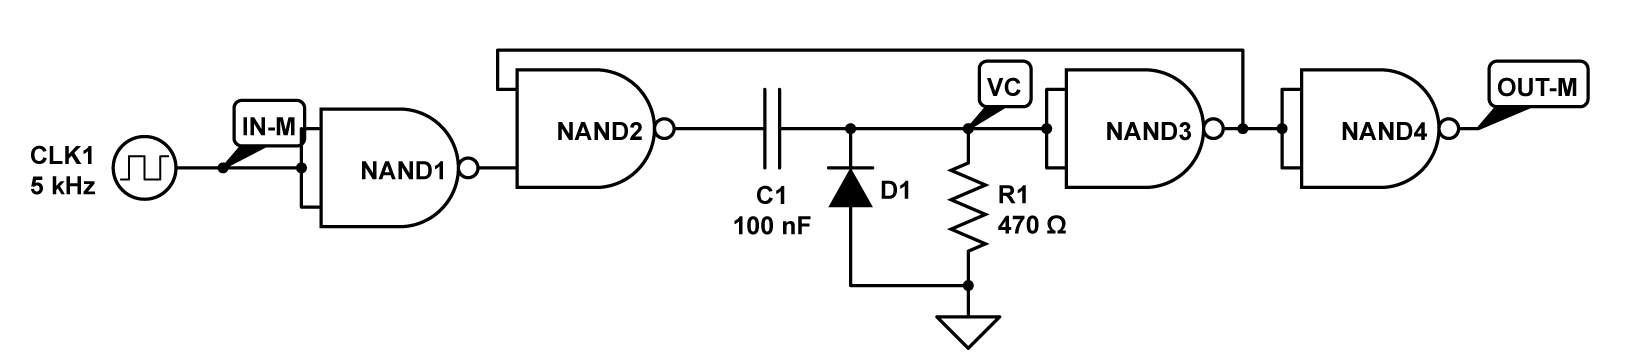
\includegraphics[scale=0.5]{monostabile.png}
	\caption{Circuito del multivibratore monostabile}
	\label{f:monostabile}
\end{figure}

\begin{figure}[h]
	\centering
	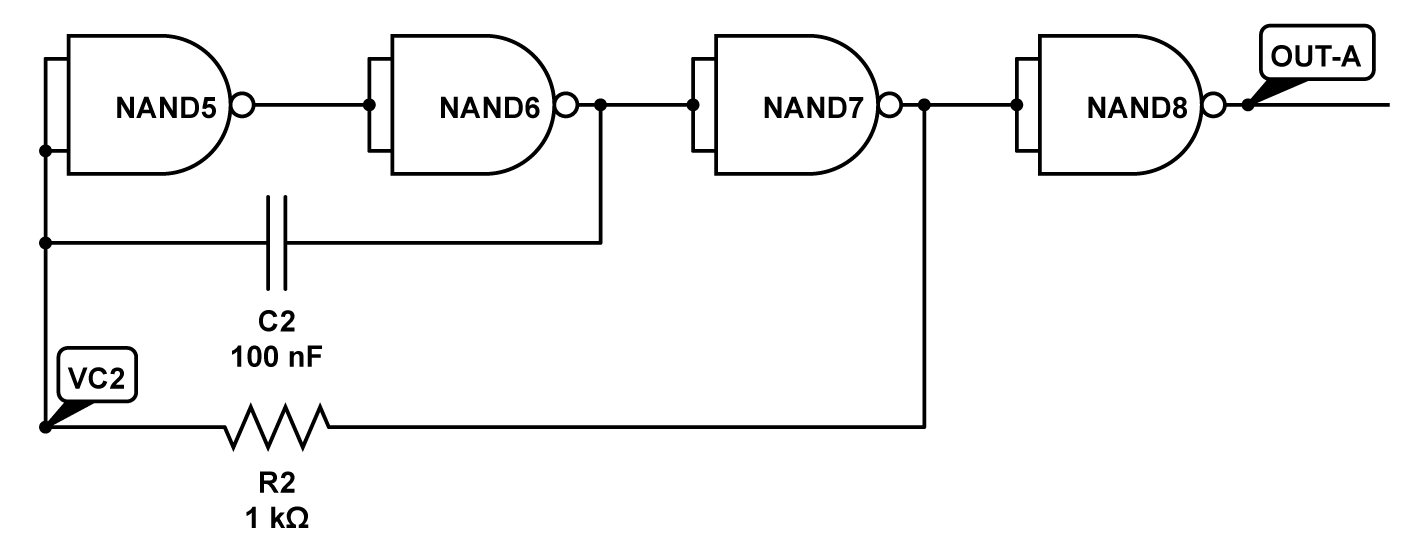
\includegraphics[scale=0.5]{astabile.png}
	\caption{Circuito del multivibratore astabile}
	\label{f:astabile}
\end{figure}

\begin{figure}[h]
	\centering
	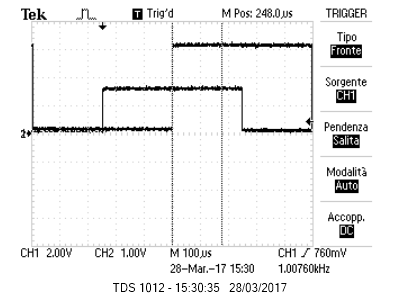
\includegraphics[scale=0.5]{ingresso.png}
	\caption{Segnali in ingresso; il segnale con il massimo minore è Y1, mentre quello con il massimo maggiore è Y2.}
	\label{f:ingressi}
\end{figure}

\begin{figure}[h]
	\centering
	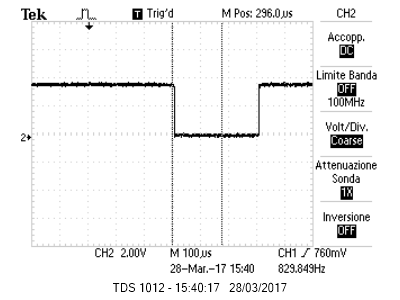
\includegraphics[scale=0.5]{nand.png}
	\caption{Uscita del circuito NAND}
	\label{f:NAND}
\end{figure}

\begin{figure}[h]
	\centering
	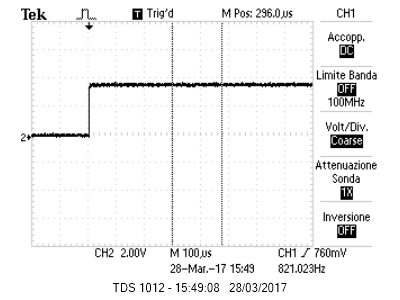
\includegraphics[scale=0.5]{or.png}
	\caption{Uscita del circuito OR}
	\label{f:OR}
\end{figure}

\begin{figure}[h]
	\centering
	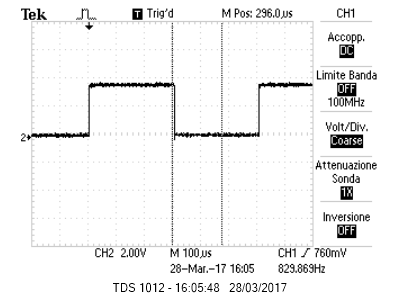
\includegraphics[scale=0.5]{xor.png}
	\caption{Uscita del circuito XOR}
	\label{f:XOR}
\end{figure}

\begin{figure}[h]
	\centering
	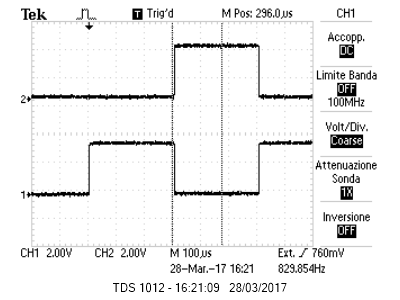
\includegraphics[scale=0.5]{sommatore.png}
	\caption{Uscite del circuito sommatore (quella superiore è il riporto, quella inferiore la somma)}
	\label{f:Sommatore}
\end{figure}